% questions.tex —— 2020 年·江苏卷 · 题目内容片段（无答案）
% 由 tools/generate_projects.py 依来源总账自 2020/2020_数学真题_江苏_试题.md 生成，勿手改（改源 MD 后重跑）


\begin{gknotice}
\textbf{来源说明}：本题面依据固定源 PDF 的两页 A3 题面逐题转录，原卷印刷页码为 1115、1116。第 1115 面为填空题 1—14、解答题 15—18；第 1116 面为解答题 19—23。原页节头只有「一、填空题」（1—14）与「二、解答题」（15—20），21 题前仅印「21．三选二．」，22、23 属附加题而无独立节头；本稿为便于检索补出「三、附加题」，题号与索引一致。所有数值、分式、根号与上下标均回原页 300—600 dpi 分栏渲染逐题核对。

\textbf{逐字核对要点}：第 6 题双曲线方程为 $\dfrac{x^2}{a^2}-\dfrac{y^2}{5}=1$（分母是 5，不是 4）；第 7 题给出的是 $f(x)=x^{\frac23}$（指数为 $\dfrac23$，不是 $\dfrac43$）；第 9 题原页体积单位印作 $\mathrm{cm}^2$，与「体积」不符，本稿照录原页，答案按体积计算；第 17 题右侧曲线关系式为 $h_2=-\dfrac1{800}b^3+6b$（$b$ 的三次方），第（2）问原文问的是「$O'E$ 为多少米」；第 20 题原页第三小问的序号误印为「（2）」，本稿按（3）编排。第 21 题原页【A】【B】【C】各小题内部仍标（1）（2），本稿一律照原样保留。

\textbf{解析归属}：固定源不附答案或解析；配套答案与解析均由本库按本题面独立复算（等级 D，非官方）。

\textbf{图形说明}：第 5 题算法流程图、第 9 题六角螺帽毛坯、第 13 题四边形 $ABPC$、第 15 题三棱柱、第 16 题 $\triangle ABC$、第 17 题桥梁竖直截面、第 22 题三棱锥 $A-BCD$，共 7 幅，均由项目内 TikZ 矢量源按原页几何重绘；其余各题原页无图。
\end{gknotice}

\gkpart{一、填空题}

\begin{question}
\gkti{1}已知集合 $A=\{-1,0,1,2\}$，$B=\{0,2,3\}$，则 $A\cap B=$\gkblank{}。

\end{question}
\begin{question}
\gkti{2}已知 $\mathrm i$ 是虚数单位，则复数 $z=(1+\mathrm i)(2-\mathrm i)$ 的实部是\gkblank{}。

\end{question}
\begin{question}
\gkti{3}已知一组数据 $4,2a,3-a,5,6$ 的平均数为 $4$，则 $a$ 的值是\gkblank{}。

\end{question}
\begin{question}
\gkti{4}将一颗质地均匀的正方体骰子先后抛掷 $2$ 次，观察向上的点数，则点数和为 $5$ 的概率是\gkblank{}。

\Needspace{0.4\textheight}
\end{question}
\begin{question}
\gkti{5}如图是一个算法流程图。若输出 $y$ 的值为 $-2$，则输入 $x$ 的值是\gkblank{}。
\nopagebreak[4]
\begin{center}% 2020 江苏卷 5：算法流程图（开始→输入 x→判断 x>0→是 y←2^x / 否 y←x+1→输出 y→结束）
% 绘制依据：固定源 PDF 第 1115 面原图。原图自上而下的主干与左「Y」右「N」的分支走向照录。
\begin{tikzpicture}[scale=0.92, font=\small, >=Stealth,
    box/.style={draw, minimum width=2.0cm, minimum height=0.72cm, align=center},
    io/.style={draw, trapezium, trapezium left angle=72, trapezium right angle=108,
      minimum width=2.2cm, minimum height=0.72cm, align=center},
    dec/.style={draw, diamond, aspect=2.1, inner sep=1pt, align=center}]
  \node[draw, rounded corners=6pt, minimum width=1.7cm, minimum height=0.72cm] (begin) at (0,0) {开始};
  \node[io] (in) at (0,-1.35) {输入 $x$};
  \node[dec] (judge) at (0,-2.85) {$x>0$?};
  \node[box] (yes) at (-2.5,-4.4) {$y\leftarrow 2^{x}$};
  \node[box] (no) at (2.5,-4.4) {$y\leftarrow x+1$};
  \node[io] (out) at (0,-5.85) {输出 $y$};
  \node[draw, rounded corners=6pt, minimum width=1.7cm, minimum height=0.72cm] (end) at (0,-7.15) {结束};

  \draw[->] (begin) -- (in);
  \draw[->] (in) -- (judge);
  \draw[->] (judge.west) -| (yes.north);
  \node at (-1.85,-2.55) {$Y$};
  \draw[->] (judge.east) -| (no.north);
  \node at (1.85,-2.55) {$N$};
  \draw[->] (yes.south) |- (out.west);
  \draw[->] (no.south) |- (out.east);
  \draw[->] (out) -- (end);
\end{tikzpicture}
\end{center}
\nopagebreak[4]
\end{question}
\begin{question}
\gkti{6}在平面直角坐标系 $xOy$ 中，若双曲线 $\dfrac{x^2}{a^2}-\dfrac{y^2}{5}=1$（$a>0$）的一条渐近线方程为 $y=\dfrac{\sqrt5}{2}x$，则该双曲线的离心率是\gkblank{}。

\end{question}
\begin{question}
\gkti{7}已知 $y=f(x)$ 是奇函数，当 $x\geqslant0$ 时，$f(x)=x^{\frac23}$，则 $f(-8)$ 的值是\gkblank{}。

\end{question}
\begin{question}
\gkti{8}已知 $\sin^2\left(\dfrac\pi4+\alpha\right)=\dfrac23$，则 $\sin2\alpha$ 的值是\gkblank{}。

\Needspace{0.4\textheight}
\end{question}
\begin{question}
\gkti{9}如图，六角螺帽毛坯是由一个正六棱柱挖去一个圆柱所构成的。已知螺帽的底面正六边形边长为 $2\ \mathrm{cm}$，高为 $2\ \mathrm{cm}$，内孔半径为 $0.5\ \mathrm{cm}$，则此六角螺帽毛坯的体积是\gkblank{}$\mathrm{cm}^2$。
\nopagebreak[4]
\begin{center}% 2020 江苏卷 9：六角螺帽毛坯（正六棱柱挖去一个圆柱）
% 绘制依据：固定源 PDF 第 1115 面原图。正六棱柱竖放，顶面为压扁的正六边形（前后各一条水平边），
% 顶面中心为一个圆柱形内孔（椭圆口），孔壁用虚线画到底面的虚线椭圆；背面棱与底面的后侧棱为虚线。
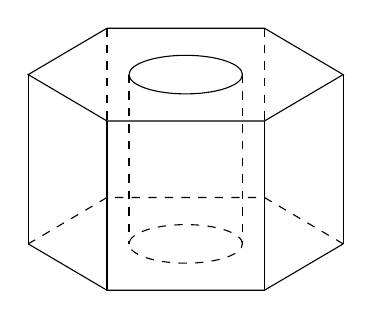
\begin{tikzpicture}[scale=1.0, font=\small]
  \def\r{2}
  \def\sq{0.34}
  \def\hh{2.15}
  % 顶面六顶点（角度 0,60,...,300），y 方向压缩为 \sq 倍
  \coordinate (P0) at ({\r*cos(0)},{\sq*\r*sin(0)});
  \coordinate (P1) at ({\r*cos(60)},{\sq*\r*sin(60)});
  \coordinate (P2) at ({\r*cos(120)},{\sq*\r*sin(120)});
  \coordinate (P3) at ({\r*cos(180)},{\sq*\r*sin(180)});
  \coordinate (P4) at ({\r*cos(240)},{\sq*\r*sin(240)});
  \coordinate (P5) at ({\r*cos(300)},{\sq*\r*sin(300)});
  % 底面六顶点：整体下移 \hh
  \coordinate (Q0) at ({\r*cos(0)},{\sq*\r*sin(0)-\hh});
  \coordinate (Q1) at ({\r*cos(60)},{\sq*\r*sin(60)-\hh});
  \coordinate (Q2) at ({\r*cos(120)},{\sq*\r*sin(120)-\hh});
  \coordinate (Q3) at ({\r*cos(180)},{\sq*\r*sin(180)-\hh});
  \coordinate (Q4) at ({\r*cos(240)},{\sq*\r*sin(240)-\hh});
  \coordinate (Q5) at ({\r*cos(300)},{\sq*\r*sin(300)-\hh});

  % 顶面轮廓（全可见，实线）
  \draw (P0) -- (P1) -- (P2) -- (P3) -- (P4) -- (P5) -- cycle;

  % 竖直棱：前面与左右两侧可见（实线），背面两条为虚线
  \draw (P0) -- (Q0);
  \draw (P3) -- (Q3);
  \draw (P4) -- (Q4);
  \draw (P5) -- (Q5);
  \draw[dashed] (P1) -- (Q1);
  \draw[dashed] (P2) -- (Q2);

  % 底面轮廓：前侧三条边可见（实线），后侧三条边被遮挡（虚线）
  \draw (Q3) -- (Q4) -- (Q5) -- (Q0);
  \draw[dashed] (Q0) -- (Q1) -- (Q2) -- (Q3);

  % 内孔：顶面椭圆口（实线），孔沿两条竖直线（虚线），底面椭圆（虚线）
  \draw (0,0) ellipse (0.72 and 0.245);
  \draw[dashed] (-0.72,0) -- (-0.72,-\hh);
  \draw[dashed] (0.72,0) -- (0.72,-\hh);
  \draw[dashed] (0,-\hh) ellipse (0.72 and 0.245);
\end{tikzpicture}
\end{center}
\nopagebreak[4]
\end{question}
\begin{question}
\gkti{10}将函数 $y=3\sin\left(2x+\dfrac\pi4\right)$ 的图象向右平移 $\dfrac\pi6$ 个单位长度，则平移后的图象中与 $y$ 轴最近的对称轴的方程是\gkblank{}。

\end{question}
\begin{question}
\gkti{11}设 $\{a_n\}$ 是公差为 $d$ 的等差数列，$\{b_n\}$ 是公比为 $q$ 的等比数列。已知数列 $\{a_n+b_n\}$ 的前 $n$ 项和 $S_n=n^2-n+2^n-1$（$n\in\mathbf N^*$），则 $d+q$ 的值是\gkblank{}。

\end{question}
\begin{question}
\gkti{12}已知 $5x^2y^2+y^4=1$（$x,y\in\mathbf R$），则 $x^2+y^2$ 的最小值是\gkblank{}。

\Needspace{0.4\textheight}
\end{question}
\begin{question}
\gkti{13}在 $\triangle ABC$ 中，$AB=4$，$AC=3$，$\angle BAC=90^\circ$，$D$ 在边 $BC$ 上，延长 $AD$ 到 $P$，使得 $AP=9$。若 $\overrightarrow{PA}=m\overrightarrow{PB}+\left(\dfrac32-m\right)\overrightarrow{PC}$（$m$ 为常数），则 $CD$ 的长度是\gkblank{}。
\nopagebreak[4]
\begin{center}% 2020 江苏卷 13：△ABC 中 D 在边 BC 上，延长 AD 到 P（AP=9）
% 绘制依据：固定源 PDF 第 1115 面原图。A 左下、B 右下、C 左上（∠BAC=90°），
% D 在 BC 上，连 PA、PB、PC（P 在右方远处）。只标 A、B、C、D、P 五点。
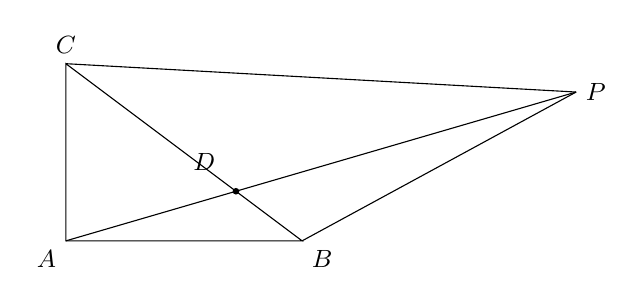
\begin{tikzpicture}[scale=0.75, font=\small]
  \coordinate (A) at (0,0);
  \coordinate (B) at (4,0);
  \coordinate (C) at (0,3);
  \coordinate (D) at (2.88,0.84);
  \coordinate (P) at (8.64,2.52);
  \draw (A) -- (B) -- (C) -- cycle;
  \draw (A) -- (P);
  \draw (B) -- (P);
  \draw (C) -- (P);
  \fill (D) circle (1.6pt);
  \node[below left] at (A) {$A$};
  \node[below right] at (B) {$B$};
  \node[above] at (C) {$C$};
  \node[above left=4pt] at (D) {$D$};
  \node[right] at (P) {$P$};
\end{tikzpicture}
\end{center}
\nopagebreak[4]
\end{question}
\begin{question}
\gkti{14}在平面直角坐标系 $xOy$ 中，已知 $P\left(\dfrac{\sqrt3}2,0\right)$，$A$，$B$ 是圆 $C:x^2+\left(y-\dfrac12\right)^2=36$ 上的两个动点，满足 $PA=PB$，则 $\triangle PAB$ 面积的最大值是\gkblank{}。

\end{question}
\gkpart{二、解答题}

\Needspace{0.4\textheight}
\begin{question}
\gkti{15}在三棱柱 $ABC-A_1B_1C_1$ 中，$AB\perp AC$，$B_1C\perp$ 平面 $ABC$，$E$，$F$ 分别是 $AC$，$B_1C$ 的中点。

（1） 求证：$EF\parallel$ 平面 $AB_1C_1$；

（2） 求证：平面 $AB_1C\perp$ 平面 $ABB_1$。
\nopagebreak[4]
\begin{center}% 2020 江苏卷 15：三棱柱 ABC-A1B1C1，E、F 分别为 AC、B1C 的中点
% 绘制依据：固定源 PDF 第 1115 面原图。斜置三棱柱：底面三角形 A 左、B 前下、C 右，
% A1、B1、C1 分别位于 A、B、C 的正上偏右（同一平移向量）。可见棱实线，隐蔽棱虚线。
% 图中另画出 AB1（实线）与 AC1（虚线，体内对角线），E 在 AC 上、F 在 B1C 上。
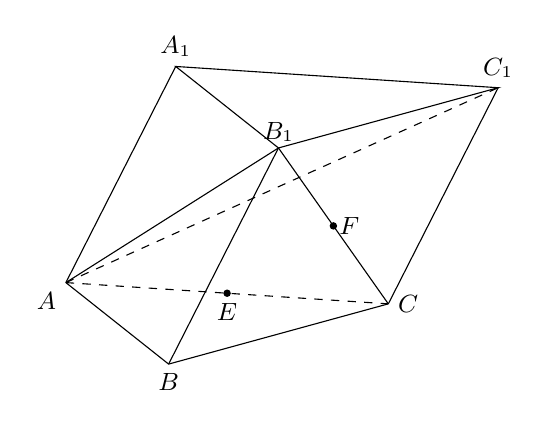
\begin{tikzpicture}[scale=0.9, font=\small]
  \coordinate (A) at (0,0);
  \coordinate (B) at (1.45,-1.15);
  \coordinate (C) at (4.55,-0.30);
  \coordinate (A1) at (1.55,3.05);
  \coordinate (B1) at (3.00,1.90);
  \coordinate (C1) at (6.10,2.75);
  \coordinate (E) at (2.275,-0.15);
  \coordinate (F) at (3.775,0.80);

  % 底面三角形
  \draw (A) -- (B) -- (C);
  \draw[dashed] (A) -- (C);
  % 侧棱
  \draw (A) -- (A1);
  \draw (B) -- (B1);
  \draw (C) -- (C1);
  % 顶面三角形
  \draw (A1) -- (B1) -- (C1) -- cycle;
  % 题设涉及的线段：AB1 实线，AC1 体内对角线（虚线），B1C 实线
  \draw (A) -- (B1);
  \draw[dashed] (A) -- (C1);
  \draw (B1) -- (C);

  \fill (E) circle (1.5pt);
  \fill (F) circle (1.5pt);
  \node[below left] at (A) {$A$};
  \node[below] at (B) {$B$};
  \node[right] at (C) {$C$};
  \node[above] at (A1) {$A_1$};
  \node[above, inner sep=2pt] at (B1) {$B_1$};
  \node[above] at (C1) {$C_1$};
  \node[below=2pt, inner sep=1.5pt] at (E) {$E$};
  \node[right, inner sep=2pt] at (F) {$F$};
\end{tikzpicture}
\end{center}
\nopagebreak[4]
\Needspace{0.4\textheight}
\end{question}
\begin{question}
\gkti{16}在 $\triangle ABC$ 中，角 $A,B,C$ 的对边分别为 $a,b,c$，已知 $a=3$，$c=\sqrt2$，$B=45^\circ$。

（1） 求 $\sin C$ 的值；

（2） 在边 $BC$ 上取一点 $D$，使得 $\cos\angle ADC=-\dfrac45$，求 $\tan\angle DAC$ 的值。
\nopagebreak[4]
\begin{center}% 2020 江苏卷 16：△ABC 中 D 在边 BC 上
% 绘制依据：固定源 PDF 第 1115 面原图。A 在上方偏右，B 左下、C 右下，D 在 BC 上靠近 C，
% 连 AD。只标 A、B、C、D 四点。
\begin{tikzpicture}[scale=1.05, font=\small]
  \coordinate (A) at (2.55,1.85);
  \coordinate (B) at (0,0);
  \coordinate (C) at (5.0,0);
  \coordinate (D) at (3.75,0);
  \draw (A) -- (B) -- (C) -- cycle;
  \draw (A) -- (D);
  \node[above] at (A) {$A$};
  \node[below left] at (B) {$B$};
  \node[below right] at (C) {$C$};
  \node[below=5pt, inner sep=3pt] at (D) {$D$};
\end{tikzpicture}
\end{center}
\nopagebreak[4]
\Needspace{0.4\textheight}
\end{question}
\begin{question}
\gkti{17}某地准备在山谷中建一座桥梁，桥址位置的竖直截面图如图所示：谷底 $O$ 在水平线 $MN$ 上，桥 $AB$ 与 $MN$ 平行，$OO'$ 为铅垂线（$O'$ 在 $AB$ 上）。经测量，左侧曲线 $AO$ 上任一点 $D$ 到 $MN$ 的距离 $h_1$（米）与 $D$ 到 $OO'$ 的距离 $a$（米）之间满足关系式 $h_1=\dfrac1{40}a^2$；右侧曲线 $BO$ 上任一点 $F$ 到 $MN$ 的距离 $h_2$（米）与 $F$ 到 $OO'$ 的距离 $b$（米）之间满足关系式 $h_2=-\dfrac1{800}b^3+6b$。已知点 $B$ 到 $OO'$ 的距离为 $40$ 米。

（1） 求桥 $AB$ 的长度；

（2） 计划在谷底两侧建造平行于 $OO'$ 的桥墩 $CD$ 和 $EF$，且 $CE$ 为 $80$ 米，其中 $C$，$E$ 在 $AB$ 上（不包括端点）。桥墩 $EF$ 每米造价 $k$（万元）、桥墩 $CD$ 每米造价 $\dfrac32k$（万元）（$k>0$）。问 $O'E$ 为多少米时，桥墩 $CD$ 与 $EF$ 的总造价最低？
\nopagebreak[4]
\begin{center}% 2020 江苏卷 17：桥梁竖直截面（谷底 O 在水平线 MN 上，桥 AB∥MN，OO' 为铅垂线）
% 绘制依据：固定源 PDF 第 1115 面原图与题给关系式 h1=a^2/40、h2=-b^3/800+6b（B 到 OO' 为 40 米）。
% 坐标换算：横向 1 米 = 0.0475 单位，纵向 1 米 = 0.0225 单位；
% 左侧 a 自 O' 向左量（a=80 时 h1=160，即 A 点），右侧 b 自 O' 向右量（b=40 时 h2=160，即 B 点）。
% 图中标出 C、D、E、F、D1、O、F1 与 a、b、h1、h2；桥墩 CD、EF 为实线，各条量距线为虚线。
\begin{tikzpicture}[scale=1.0, font=\small]
  \def\ox{4.6}      % O' 的横坐标
  \def\ky{0.0225}   % 纵向比例（米 -> 单位）
  \def\kx{0.0475}   % 横向比例（米 -> 单位）
  \def\H{3.6}       % 桥面高 160 米

  % 水平线 MN
  \draw (-0.55,0) -- (8.3,0);
  \node[below] at (-0.45,0) {$M$};
  \node[below] at (8.2,0) {$N$};

  % 左曲线 h1=a^2/40（a 自 O' 向左量），绘到 A 点上方
  \draw[thick] plot[domain=0:92, samples=140]
    ({\ox-\kx*\x}, {\ky*\x*\x/40});
  % 右曲线 h2=-b^3/800+6b（b 自 O' 向右量），绘过 B 点后再下垂
  \draw[thick] plot[domain=0:46, samples=160]
    ({\ox+\kx*\x}, {\ky*(-0.00125*\x*\x*\x+6*\x)});

  % 桥面 AB（水平，与 MN 平行）
  \draw (0.80,\H) -- (6.50,\H);

  % 铅垂线 OO'
  \draw[dashed] (\ox,0) -- (\ox,\H);

  % 桥墩 CD：C 在桥面上，D 在左曲线（a=60 米）
  \draw (1.75,\H) -- (1.75,2.025);
  % 桥墩 EF：E 在桥面上，F 在右曲线（b=20 米）
  \draw (5.55,\H) -- (5.55,2.475);

  % D、F 到 MN 的虚线（h1、h2）
  \draw[dashed] (1.75,2.025) -- (1.75,0);
  \draw[dashed] (5.55,2.475) -- (5.55,0);
  % 量距 a、b 的虚线
  \draw[dashed] (1.75,2.025) -- (\ox,2.025);
  \draw[dashed] (5.55,2.475) -- (\ox,2.475);

  % 标注
  \node at (0.40,3.72) {$A$};
  \node[above] at (1.75,\H) {$C$};
  \node[above] at (\ox,\H) {$O'$};
  \node[above] at (5.55,\H) {$E$};
  \node at (6.62,3.80) {$B$};
  \node[left] at (1.72,2.03) {$D$};
  \node[right] at (5.58,2.44) {$F$};
  \node[below] at (1.75,0) {$D_1$};
  \node[below] at (\ox,0) {$O$};
  \node[below] at (5.55,0) {$F_1$};
  \node at (3.20,1.88) {$a$};
  \node at (5.02,2.70) {$b$};
  \node at (1.42,1.02) {$h_1$};
  \node at (5.92,1.42) {$h_2$};
\end{tikzpicture}
\end{center}
\nopagebreak[4]
\end{question}
\begin{question}
\gkti{18}在平面直角坐标系 $xOy$ 中，已知椭圆 $E:\dfrac{x^2}4+\dfrac{y^2}3=1$ 的左、右焦点分别为 $F_1$，$F_2$，点 $A$ 在椭圆 $E$ 上且在第一象限内，$AF_2\perp F_1F_2$，直线 $AF_1$ 与椭圆 $E$ 相交于另一点 $B$。

（1） 求 $\triangle AF_1F_2$ 的周长；

（2） 在 $x$ 轴上任取一点 $P$，直线 $AP$ 与椭圆 $E$ 的右准线相交于点 $Q$，求 $\overrightarrow{OP}\cdot\overrightarrow{QP}$ 的最小值；

（3） 设点 $M$ 在椭圆 $E$ 上，记 $\triangle OAB$ 与 $\triangle MAB$ 的面积分别为 $S_1$，$S_2$，若 $S_2=3S_1$，求点 $M$ 的坐标。

\end{question}
\begin{question}
\gkti{19}已知关于 $x$ 的函数 $y=f(x)$，$y=g(x)$ 与 $h(x)=kx+b$（$k,b\in\mathbf R$）在区间 $D$ 上恒有 $f(x)\geqslant h(x)\geqslant g(x)$。

（1） 若 $f(x)=x^2+2x$，$g(x)=-x^2+2x$，$D=(-\infty,+\infty)$，求 $h(x)$ 的表达式；

（2） 若 $f(x)=x^2-x+1$，$g(x)=k\ln x$，$h(x)=kx-k$，$D=(0,+\infty)$，求 $k$ 的取值范围；

（3） 若 $f(x)=x^4-2x^2$，$g(x)=4x^2-8$，$h(x)=4(t^3-t)x-3t^4+2t^2$（$0<|t|\leqslant\sqrt2$），$D=[m,n]\subseteq[-\sqrt2,\sqrt2]$，求证：$n-m\leqslant\sqrt7$。

\end{question}
\begin{question}
\gkti{20}已知数列 $\{a_n\}$（$n\in\mathbf N^*$）的首项 $a_1=1$，前 $n$ 项和为 $S_n$。设 $\lambda$ 与 $k$ 是常数，若对一切正整数 $n$，均有 $S_{n+1}^{\frac1k}-S_n^{\frac1k}=\lambda a_{n+1}^{\frac1k}$ 成立，则称此数列为「$\lambda\sim k$」数列。

（1） 若等差数列 $\{a_n\}$ 是「$\lambda\sim1$」数列，求 $\lambda$ 的值；

（2） 若数列 $\{a_n\}$ 是「$\dfrac{\sqrt3}3\sim2$」数列，且 $a_n>0$，求数列 $\{a_n\}$ 的通项公式；

（3） 对于给定的 $\lambda$，是否存在三个不同的数列 $\{a_n\}$ 为「$\lambda\sim3$」数列，且 $a_n\geqslant0$？若存在，求 $\lambda$ 的取值范围；若不存在，说明理由。

\end{question}
\gkpart{三、附加题}

\begin{question}
\gkti{21}选做（三选二）。

\textbf{【A】} 平面上点 $A(2,-1)$ 在矩阵 $\boldsymbol M=\begin{bmatrix}a&1\\-1&b\end{bmatrix}$ 对应的变换作用下得到点 $B(3,-4)$。（1） 求实数 $a$，$b$ 的值；（2） 求矩阵 $\boldsymbol M$ 的逆矩阵 $\boldsymbol M^{-1}$。

\textbf{【B】} 在极坐标系中，已知点 $A\left(\rho_1,\dfrac\pi3\right)$ 在直线 $l:\rho\cos\theta=2$ 上，点 $B\left(\rho_2,\dfrac\pi6\right)$ 在圆 $C:\rho=4\sin\theta$ 上（其中 $\rho\geqslant0$，$0\leqslant\theta<2\pi$）。（1） 求 $\rho_1$，$\rho_2$ 的值；（2） 求出直线 $l$ 与圆 $C$ 的公共点的极坐标。

\textbf{【C】} 设 $x\in\mathbf R$，解不等式 $2|x+1|+|x|\leqslant4$。

\Needspace{0.4\textheight}
\end{question}
\begin{question}
\gkti{22}在三棱锥 $A-BCD$ 中，已知 $CB=CD=\sqrt5$，$BD=2$，$O$ 为 $BD$ 的中点，$AO\perp$ 平面 $BCD$，$AO=2$，$E$ 为 $AC$ 的中点。

（1） 求直线 $AB$ 与 $DE$ 所成角的余弦值；

（2） 若点 $F$ 在 $BC$ 上，满足 $BF=\dfrac14BC$，设二面角 $F-DE-C$ 的大小为 $\theta$，求 $\sin\theta$ 的值。
\nopagebreak[4]
\begin{center}% 2020 江苏卷 22：三棱锥 A-BCD，O 为 BD 中点，E 为 AC 中点，F 在 BC 上（BF=BC/4）
% 绘制依据：固定源 PDF 第 1116 面原图。A 在上，B 左下，C 右，D 在内部（被遮挡），
% 可见棱 AB、AC（含 AE、EC）、BC（含 BF、FC）与面 ABC 内的 EF 为实线；
% 隐蔽棱 AD、AO、BD（含 BO、OD）、DC、DE 为虚线。标出 A、B、C、D、O、E、F。
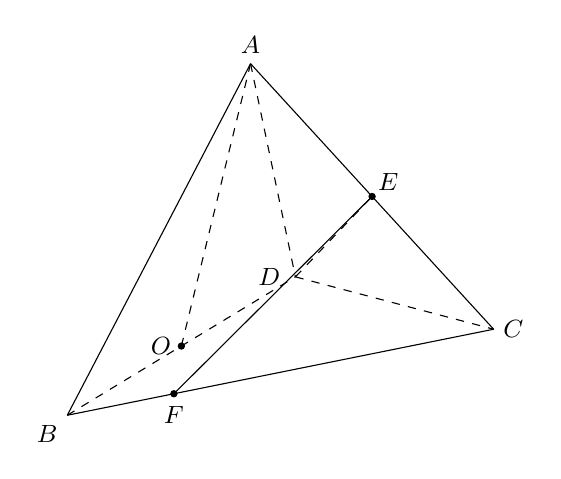
\begin{tikzpicture}[scale=0.95, font=\small]
  \coordinate (A) at (2.45,4.70);
  \coordinate (B) at (0.00,0.00);
  \coordinate (C) at (5.70,1.15);
  \coordinate (D) at (3.05,1.85);
  \coordinate (O) at (1.525,0.925);
  \coordinate (E) at (4.075,2.925);
  \coordinate (F) at (1.425,0.2875);

  % 可见棱
  \draw (A) -- (B);
  \draw (A) -- (E) -- (C);
  \draw (B) -- (F) -- (C);
  \draw (E) -- (F);
  % 隐蔽棱
  \draw[dashed] (A) -- (D);
  \draw[dashed] (A) -- (O);
  \draw[dashed] (B) -- (D);
  \draw[dashed] (D) -- (C);
  \draw[dashed] (D) -- (E);

  \fill (O) circle (1.4pt);
  \fill (E) circle (1.4pt);
  \fill (F) circle (1.4pt);
  \node[above] at (A) {$A$};
  \node[below left] at (B) {$B$};
  \node[right] at (C) {$C$};
  \node[left=2pt] at (D) {$D$};
  \node[left=1pt, inner sep=2.5pt] at (O) {$O$};
  \node[above right, inner sep=2pt] at (E) {$E$};
  \node[below=2pt, inner sep=2.5pt] at (F) {$F$};
\end{tikzpicture}
\end{center}
\nopagebreak[4]
\end{question}
\begin{question}
\gkti{23}甲口袋中装有 $2$ 个黑球和 $1$ 个白球，乙口袋中装有 $3$ 个白球。现从甲、乙两口袋中各任取一个球交换放入另一口袋，重复 $n$ 次这样的操作，记甲口袋中黑球个数为 $X_n$，恰有 $2$ 个黑球的概率为 $p_n$，恰有 $1$ 个黑球的概率为 $q_n$。

（1） 求 $p_1$，$q_1$ 和 $p_2$，$q_2$；

（2） 求 $2p_n+q_n$ 与 $2p_{n-1}+q_{n-1}$ 的递推关系式和 $X_n$ 的数学期望 $E(X_n)$（用 $n$ 表示）。

\end{question}